\subsection{协方差与相关}\label{sec:4.5}
前面几节讨论了两个随机变量之间有无关系，即独立或不独立. 但即便存在关系，也可能有强有弱. 本节讨论度量两个随机变量关系强弱的两个数值指标：协方差与相关.

为说明两个随机变量之间关系的强弱是什么意思，考虑两个不同的实验. 在第一个实验中，测量随机变量 $X,Y$：$X$ 是一份水样的重量，$Y$ 是同一水样的体积. 显然，$X$ 与 $Y$ 有很强的关系. 对若干水样测量 $(X,Y)$，并将观测数据对画出来，由于二者的物理关系，数据点应落在一条直线上. 测量误差、水中杂质等因素会使它们不能精确地落在直线上，但只要实验操作足够细致，这些点就会非常接近一条直线. 再考虑另一个实验：$X$ 是某人的体重，$Y$ 是同一个人的身高. 二者显然也存在关系，但远没有前一个实验那么强. 我们不会期望不同人的 $(X,Y)$ 数据对排成一条直线，尽管可能预期图中呈现上升趋势. 协方差与相关就是将这种关系强弱的差别数量化的两个指标.

本节将经常涉及 $X$ 的均值和方差，以及 $Y$ 的均值和方差. 使用记号 $EX=\mu_X$、$EY=\mu_Y$、$\operatorname{Var}X=\sigma_X^2$、$\operatorname{Var}Y=\sigma_Y^2$. 始终假定 $0<\sigma_X^2<\infty$，$0<\sigma_Y^2<\infty$.
\begin{definition}\label{def:4.5.1}\index{SI0223@协方差（另见相关）}
$X$ 和 $Y$ 的协方差（covariance）定义为
$$\operatorname{Cov}(X,Y)=E((X-\mu_X)(Y-\mu_Y)).$$
\end{definition}
\sourcepageanchor{170}

\begin{definition}\label{def:4.5.2}\index{SI0216@系数}\index{SI0217@相关（另见协方差）}
$X$ 和 $Y$ 的相关（correlation）定义为
$$\rho_{XY}=\frac{\operatorname{Cov}(X,Y)}{\sigma_X\sigma_Y}.$$
数值 $\rho_{XY}$ 也称为相关系数（correlation coefficient）.
\end{definition}
如果 $X$ 的大值往往与 $Y$ 的大值一起出现，$X$ 的小值往往与 $Y$ 的小值一起出现，则 $\operatorname{Cov}(X,Y)$ 为正. 若 $X>\mu_X$，则很可能 $Y>\mu_Y$，于是乘积 $(X-\mu_X)(Y-\mu_Y)$ 为正. 若 $X<\mu_X$，则很可能 $Y<\mu_Y$，这个乘积仍为正. 所以 $\operatorname{Cov}(X,Y)=E((X-\mu_X)(Y-\mu_Y))>0$. 如果 $X$ 的大值往往与 $Y$ 的小值一起出现，而 $X$ 的小值与 $Y$ 的大值一起出现，则协方差为负，因为 $X>\mu_X$ 时，$Y$ 往往小于 $\mu_Y$，反之亦然，所以 $(X-\mu_X)(Y-\mu_Y)$ 往往为负. 因而，协方差的符号提供了关于 $X,Y$ 关系的信息.

但是，$\operatorname{Cov}(X,Y)$ 可以取任意数值；仅仅知道一个给定值，例如 $\operatorname{Cov}(X,Y)=3$，本身不能说明关系有多强. 另一方面，相关系数总在 $-1$ 与 1 之间，取 $-1$ 或 1 表示 $X$ 与 $Y$ 之间有完全线性关系. \autoref{thm:4.5.7} 将证明这一点.

在考察协方差与相关的这些性质之前，先在一个具体例子中计算它们. 下述结论将简化计算.
\begin{theorem}\label{thm:4.5.3}
对任意随机变量 $X$ 和 $Y$，
$$\operatorname{Cov}(X,Y)=EXY-\mu_X\mu_Y.$$
\end{theorem}
\begin{proof}
$$\begin{aligned}
\operatorname{Cov}(X,Y)&=E((X-\mu_X)(Y-\mu_Y))\\
&=E(XY-\mu_XY-\mu_YX+\mu_X\mu_Y)&&\text{（展开乘积）}\\
&=EXY-\mu_XEY-\mu_YEX+\mu_X\mu_Y&&\text{（$\mu_X,\mu_Y$ 为常数）}\\
&=EXY-\mu_X\mu_Y-\mu_Y\mu_X+\mu_X\mu_Y\\
&=EXY-\mu_X\mu_Y.
\end{aligned}$$
\end{proof}
\begin{example}[相关——I]\label{ex:4.5.4}
设 $(X,Y)$ 的联合 pdf 为 $f(x,y)=1$，$0<x<1$，$x<y<x+1$. $X$ 的边缘分布是 $\operatorname{uniform}(0,1)$，所以 $\mu_X=1/2$，$\sigma_X^2=1/12$. $Y$ 的边缘 pdf 为 $f_Y(y)=y$（$0<y<1$）及 $f_Y(y)=2-y$（$1\le y<2$），且 $\mu_Y=1$，$\sigma_Y^2=1/6$. 还有
$$\begin{aligned}
EXY&=\int_0^1\int_x^{x+1}xy\,dy\,dx=\int_0^1\left.\frac12xy^2\right|_x^{x+1}\,dx\\
&=\int_0^1\left(x^2+\frac12x\right)\,dx=\frac7{12}.
\end{aligned}$$
由\autoref{thm:4.5.3}，$\operatorname{Cov}(X,Y)=7/12-(1/2)(1)=1/12$. 相关系数为
$$\rho_{XY}=\frac{\operatorname{Cov}(X,Y)}{\sigma_X\sigma_Y}=\frac{1/12}{\sqrt{1/12}\sqrt{1/6}}=\frac1{\sqrt2}.$$
\end{example}
接下来三个定理描述协方差与相关的一些基本性质.
\sourcepageanchor{171}

\begin{theorem}\label{thm:4.5.5}\index{SI0221@独立性}\index{SI0548@协方差}
如果 $X$ 和 $Y$ 是独立随机变量，则 $\operatorname{Cov}(X,Y)=0$，$\rho_{XY}=0$.
\end{theorem}
\begin{proof}
因为 $X$ 与 $Y$ 独立，由\autoref{thm:4.2.10}，$EXY=(EX)(EY)$. 所以
$$\operatorname{Cov}(X,Y)=EXY-(EX)(EY)=(EX)(EY)-(EX)(EY)=0,$$
且
$$\rho_{XY}=\frac{\operatorname{Cov}(X,Y)}{\sigma_X\sigma_Y}=\frac0{\sigma_X\sigma_Y}=0.$$
\end{proof}
因此，在某种意义上，$\operatorname{Cov}(X,Y)=\rho_{XY}=0$ 表示 $X$ 与 $Y$ 没有关系. 但必须注意，\autoref{thm:4.5.5} 并没有说协方差为 0 就意味着独立. 例如，设 $X\sim f(x-\theta)$，关于 0 对称，且 $EX=\theta$；令 $Y$ 为示性函数 $Y=I(|X-\theta|<2)$，则 $X$ 和 $Y$ 显然不独立.\footnote{译注：原文“关于 0 对称”应指基准密度 $f(t)$；$X$ 的密度 $f(x-\theta)$ 是关于 $\theta$ 对称. 此外，断言不独立还需 $0<P(|X-\theta|<2)<1$，否则 $Y$ 为常数.} 然而，
$$\begin{aligned}
E(XY)&=\int_{-\infty}^{\infty}xI(|x-\theta|<2)f(x-\theta)\,dx\\
&=\int_{-2}^2(t+\theta)f(t)\,dt=\theta\int_{-2}^2f(t)\,dt=EXEY,
\end{aligned}$$
其中利用了对称性给出的 $\int_{-2}^2tf(t)\,dt=0$. 可见，找到不相关但不独立的随机变量并不困难.

协方差与相关只度量一种特定的线性关系，\autoref{thm:4.5.7} 将进一步说明. 另见\autoref{ex:4.5.9}：两个随机变量关系很强，但由于关系不是线性的，协方差与相关都为 0.

协方差还在理解随机变量之和的变异方面起重要作用，下面这个对\autoref{thm:2.3.4} 的推广说明了这一点. 更进一步的推广见\autoref{exercise:4.44}.
\begin{theorem}\label{thm:4.5.6}\index{SI1068@和}
若 $X,Y$ 为任意两个随机变量，$a,b$ 为任意两个常数，则
$$\operatorname{Var}(aX+bY)=a^2\operatorname{Var}X+b^2\operatorname{Var}Y+2ab\operatorname{Cov}(X,Y).$$
若 $X$ 和 $Y$ 独立，则
$$\operatorname{Var}(aX+bY)=a^2\operatorname{Var}X+b^2\operatorname{Var}Y.$$
\end{theorem}
\begin{proof}
$aX+bY$ 的均值为 $E(aX+bY)=aEX+bEY=a\mu_X+b\mu_Y$. 因此，
$$\begin{aligned}
\operatorname{Var}(aX+bY)&=E\bigl[((aX+bY)-(a\mu_X+b\mu_Y))^2\bigr]\\
&=E\bigl[(a(X-\mu_X)+b(Y-\mu_Y))^2\bigr]\\
&=E\bigl[a^2(X-\mu_X)^2+b^2(Y-\mu_Y)^2+2ab(X-\mu_X)(Y-\mu_Y)\bigr]\\
&=a^2E(X-\mu_X)^2+b^2E(Y-\mu_Y)^2+2abE((X-\mu_X)(Y-\mu_Y))\\
&=a^2\operatorname{Var}X+b^2\operatorname{Var}Y+2ab\operatorname{Cov}(X,Y).
\end{aligned}$$
若 $X$ 与 $Y$ 独立，由\autoref{thm:4.5.5} 有 $\operatorname{Cov}(X,Y)=0$，第二个等式立即由第一个得到.
\end{proof}
根据\autoref{thm:4.5.6}，如果 $X$ 和 $Y$ 正相关（$\operatorname{Cov}(X,Y)>0$），则 $X+Y$ 的变异大于 $X,Y$ 各自变异之和. 如果二者负相关，则 $X+Y$ 的变异小于这个和. 对负相关随机变量，一个的大值往往伴随另一个的小值，求和时两个极端相互抵消. 所得 $X+Y$ 往往没有那么多极端值，因而方差较小. 取 $a=1$、$b=-1$，便得到两个随机变量之差的方差表达式，同样可以作类似解释.

下述定理在一定程度上说明了协方差与相关所度量的线性关系的性质.
\sourcepageanchor{172}

\begin{theorem}\label{thm:4.5.7}\index{SI0217@相关（另见协方差）}\index{SI0564@Cauchy–Schwarz}
对任意随机变量 $X$ 和 $Y$，
\begin{enumerate}
\item[(a)] $-1\le\rho_{XY}\le1$.
\item[(b)] $|\rho_{XY}|=1$ 当且仅当存在数 $a\ne0$ 与 $b$，使 $P(Y=aX+b)=1$. 如果 $\rho_{XY}=1$，则 $a>0$；如果 $\rho_{XY}=-1$，则 $a<0$.
\end{enumerate}
\end{theorem}
\begin{proof}
考虑函数
$$h(t)=E\bigl[((X-\mu_X)t+(Y-\mu_Y))^2\bigr].$$
展开得到
$$\begin{aligned}
h(t)&=t^2E(X-\mu_X)^2+2tE((X-\mu_X)(Y-\mu_Y))+E(Y-\mu_Y)^2\\
&=t^2\sigma_X^2+2t\operatorname{Cov}(X,Y)+\sigma_Y^2.
\end{aligned}$$
这个关于 $t$ 的二次函数对所有 $t$ 均大于或等于 0，因为它是非负随机变量的期望. 所以它至多有一个实根，判别式必不为正，即
$$(2\operatorname{Cov}(X,Y))^2-4\sigma_X^2\sigma_Y^2\le0.$$
这等价于
$$-\sigma_X\sigma_Y\le\operatorname{Cov}(X,Y)\le\sigma_X\sigma_Y.$$
除以 $\sigma_X\sigma_Y$，得到
$$-1\le\frac{\operatorname{Cov}(X,Y)}{\sigma_X\sigma_Y}=\rho_{XY}\le1.$$
此外，$|\rho_{XY}|=1$ 当且仅当判别式为 0，也就是 $h(t)$ 恰有一个实根. 由于 $((X-\mu_X)t+(Y-\mu_Y))^2\ge0$，期望 $h(t)=E[((X-\mu_X)t+(Y-\mu_Y))^2]=0$ 当且仅当
$$P([(X-\mu_X)t+(Y-\mu_Y)]^2=0)=1.$$
这又等价于
$$P((X-\mu_X)t+(Y-\mu_Y)=0)=1.$$
取 $a=-t$、$b=\mu_Xt+\mu_Y$，其中 $t$ 是 $h(t)$ 的根，即得 $P(Y=aX+b)=1$. 根据二次方程求根公式，这个根为 $t=-\operatorname{Cov}(X,Y)/\sigma_X^2$. 因此，$a=-t$ 与 $\rho_{XY}$ 同号，最后一个断言也得证.
\end{proof}
在\autoref{sec:4.7} 中，将证明一个称为 Cauchy--Schwarz 不等式的定理. 直接应用它就能得到 $\rho_{XY}$ 介于 $-1$ 和 1 之间；我们会看到，使用它可以缩短上面的证明.

如果存在直线 $y=ax+b$，$a\ne0$，使 $(X,Y)$ 的取值有很高概率位于该直线附近，那么 $X,Y$ 的相关系数就接近 1 或 $-1$. 如果不存在这样的直线，相关系数就接近 0. 这是对相关所度量的线性关系的一种直观理解. 下面两个例子将进一步说明.
\begin{example}[相关——II]\label{ex:4.5.8}
本例与\autoref{ex:4.5.4} 类似，但采用不同的推导方式，以说明其他建模和计算技巧. 设 $X$ 服从 $\operatorname{uniform}(0,1)$，$Z$ 服从 $\operatorname{uniform}(0,1/10)$，且 $X$ 与 $Z$ 独立. 令 $Y=X+Z$，考虑随机向量 $(X,Y)$. 可以利用\autoref{sec:4.3} 的方法，从 $(X,Z)$ 的联合分布推得 $(X,Y)$ 的联合分布. $(X,Y)$ 的联合 pdf 为
$$f(x,y)=10,\qquad0<x<1,\quad x<y<x+\frac1{10}.$$
\sourcepageanchor{173}

\begin{figure}[htbp]
\centering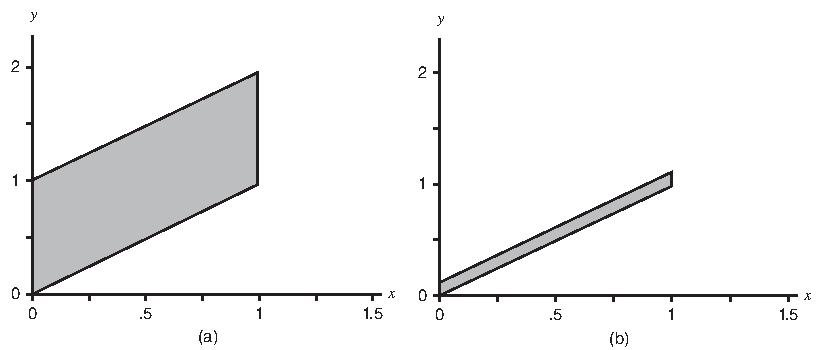
\includegraphics[width=.94\linewidth]{assets/chapter4/fig4-5-1.pdf}
\caption{(a) \autoref{ex:4.5.4} 中 $f(x,y)>0$ 的区域；(b) \autoref{ex:4.5.8} 中 $f(x,y)>0$ 的区域}\label{fig:4.5.1}
\end{figure}

无须使用\autoref{sec:4.3} 的正式方法，也可如下说明. 给定 $X=x$，有 $Y=x+Z$. 由于 $X$ 与 $Z$ 独立，给定 $X=x$ 时 $Z$ 的条件分布仍为 $\operatorname{uniform}(0,1/10)$. 因此，$x$ 在 $Y\mid X=x$ 的条件分布中充当位置参数，这个条件分布就是 $\operatorname{uniform}(x,x+1/10)$. 将此条件 pdf 与 $X$ 的边缘 pdf（$\operatorname{uniform}(0,1)$）相乘，便得到上述联合 pdf. 表示式 $Y=X+Z$ 使协方差与相关的计算很容易. $X,Y$ 的期望分别为 $EX=1/2$ 和 $EY=E(X+Z)=EX+EZ=1/2+1/20=11/20$，因此
$$\begin{aligned}
\operatorname{Cov}(X,Y)&=EXY-(EX)(EY)\\
&=E[X(X+Z)]-(EX)(E(X+Z))\\
&=EX^2+EXZ-(EX)^2-(EX)(EZ)\\
&=EX^2-(EX)^2+(EX)(EZ)-(EX)(EZ)&&\text{（$X,Z$ 独立）}\\
&=\sigma_X^2=\frac1{12}.
\end{aligned}$$
根据\autoref{thm:4.5.6}，$Y$ 的方差为 $\sigma_Y^2=\operatorname{Var}(X+Z)=\operatorname{Var}X+\operatorname{Var}Z=1/12+1/1200$. 所以
$$\rho_{XY}=\frac{1/12}{\sqrt{1/12}\sqrt{1/12+1/1200}}=\sqrt{\frac{100}{101}}.$$
这比\autoref{ex:4.5.4} 中的 $\rho_{XY}=1/\sqrt2$ 大得多. \autoref{fig:4.5.1} 展示了\autoref{ex:4.5.4} 和本例中 $f(x,y)$ 为正的集合. 回顾，这个集合称为分布的支撑集（support）. 两种情形中，$(X,Y)$ 都是相应集合中的随机点，且 $X,Y$ 都有线性递增关系. 但\hyperref[fig:4.5.1]{图 4.5.1(b)} 中的关系强得多. 还可以这样理解：本例中，$Y\mid X=x$ 的条件分布为 $\operatorname{uniform}(x,x+1/10)$；\autoref{ex:4.5.4} 中则为 $\operatorname{uniform}(x,x+1)$. 在本模型中，知道 $X=x$ 能提供比\autoref{ex:4.5.4} 多得多的关于 $Y$ 值的信息，因此相关系数更接近 1.
\end{example}
下例说明，即便 $X,Y$ 的关系很强，如果关系不是线性的，相关系数仍可能很小.
\sourcepageanchor{174}

\begin{figure}[htbp]
\centering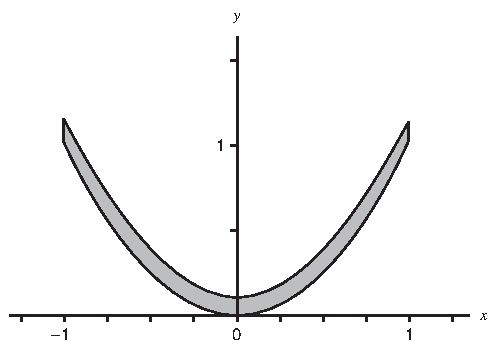
\includegraphics[width=.65\linewidth]{assets/chapter4/fig4-5-2.pdf}
\caption{\autoref{ex:4.5.9} 中 $f(x,y)>0$ 的区域}\label{fig:4.5.2}
\end{figure}

\begin{example}[相关——III]\label{ex:4.5.9}
设 $X$ 服从 $\operatorname{uniform}(-1,1)$，$Z$ 服从 $\operatorname{uniform}(0,1/10)$，且 $X$ 与 $Z$ 独立. 令 $Y=X^2+Z$，考虑随机向量 $(X,Y)$. 与\autoref{ex:4.5.8} 一样，给定 $X=x$ 时，$Y=x^2+Z$，所以 $Y\mid X=x$ 的条件分布是 $\operatorname{uniform}(x^2,x^2+1/10)$. 此条件 pdf 与 $X$ 的边缘 pdf 之积给出联合 pdf：
$$f(x,y)=5,\qquad-1<x<1,\quad x^2<y<x^2+\frac1{10}.$$
\autoref{fig:4.5.2} 展示了 $f(x,y)>0$ 的集合. 从给定 $X=x$ 时 $Y$ 的条件分布可见，$X,Y$ 的关系很强，但不是线性的. $(X,Y)$ 的可能值聚集在一条抛物线附近，而不是直线附近. 相关系数不度量这种非线性关系；事实上，$\rho_{XY}=0$. 因为 $X\sim\operatorname{uniform}(-1,1)$，有 $EX=EX^3=0$；又因为 $X,Z$ 独立，$EXZ=(EX)(EZ)$. 因此，
$$\begin{aligned}
\operatorname{Cov}(X,Y)&=E[X(X^2+Z)]-(EX)(E(X^2+Z))\\
&=EX^3+EXZ-0E(X^2+Z)\\
&=0+(EX)(EZ)=0(EZ)=0,
\end{aligned}$$
且 $\rho_{XY}=\operatorname{Cov}(X,Y)/(\sigma_X\sigma_Y)=0$.
\end{example}
本节最后引入一个非常重要的二元分布，其中相关系数自然地作为参数出现.
\begin{definition}\label{def:4.5.10}\index{SI0273@二元正态}
设 $-\infty<\mu_X<\infty$、$-\infty<\mu_Y<\infty$、$0<\sigma_X$、$0<\sigma_Y$、$-1<\rho<1$ 为五个实数. 均值为 $\mu_X,\mu_Y$，方差为 $\sigma_X^2,\sigma_Y^2$，相关系数为 $\rho$ 的二元正态 pdf（bivariate normal pdf）定义为
$$\begin{aligned}
f(x,y)&=\left(2\pi\sigma_X\sigma_Y\sqrt{1-\rho^2}\right)^{-1}\\
&\,\times\exp\left\{-\frac1{2(1-\rho^2)}\left[\left(\frac{x-\mu_X}{\sigma_X}\right)^2
-2\rho\left(\frac{x-\mu_X}{\sigma_X}\right)\left(\frac{y-\mu_Y}{\sigma_Y}\right)
+\left(\frac{y-\mu_Y}{\sigma_Y}\right)^2\right]\right\},
\end{aligned}$$
其中 $-\infty<x<\infty$，$-\infty<y<\infty$.
\end{definition}
\sourcepageanchor{175}

虽然二元正态 pdf 的公式看起来很吓人，它却是使用最频繁的二元分布之一. 实际上，公式的推导完全可以不那么吓人，见\autoref{exercise:4.46}.

此分布有许多良好性质，包括：
\begin{enumerate}
\item[(a)]\phantomsection\label{itm:bivnormal:a} $X$ 的边缘分布为 $n(\mu_X,\sigma_X^2)$.
\item[(b)]\phantomsection\label{itm:bivnormal:b} $Y$ 的边缘分布为 $n(\mu_Y,\sigma_Y^2)$.
\item[(c)]\phantomsection\label{itm:bivnormal:c} $X,Y$ 之间的相关系数为 $\rho_{XY}=\rho$.
\item[(d)]\phantomsection\label{itm:bivnormal:d} 对任意常数 $a,b$，$aX+bY$ 的分布为 $n(a\mu_X+b\mu_Y,a^2\sigma_X^2+b^2\sigma_Y^2+2ab\rho\sigma_X\sigma_Y)$.
\end{enumerate}
性质 \hyperref[itm:bivnormal:a]{(a)}、\hyperref[itm:bivnormal:b]{(b)}、\hyperref[itm:bivnormal:d]{(d)} 的验证留作习题（\autoref{exercise:4.45}）. 假设 \hyperref[itm:bivnormal:a]{(a)}、\hyperref[itm:bivnormal:b]{(b)} 成立，下面证明 \hyperref[itm:bivnormal:c]{(c)}. 由定义，
$$\begin{aligned}
\rho_{XY}&=\frac{\operatorname{Cov}(X,Y)}{\sigma_X\sigma_Y}
=\frac{E((X-\mu_X)(Y-\mu_Y))}{\sigma_X\sigma_Y}\\
&=E\left[\left(\frac{X-\mu_X}{\sigma_X}\right)\left(\frac{Y-\mu_Y}{\sigma_Y}\right)\right]\\
&=\int_{-\infty}^{\infty}\int_{-\infty}^{\infty}\left(\frac{x-\mu_X}{\sigma_X}\right)\left(\frac{y-\mu_Y}{\sigma_Y}\right)f(x,y)\,dx\,dy.
\end{aligned}$$
作变量替换
$$s=\left(\frac{x-\mu_X}{\sigma_X}\right)\left(\frac{y-\mu_Y}{\sigma_Y}\right),\qquad t=\frac{x-\mu_X}{\sigma_X}.$$
则 $x=\sigma_Xt+\mu_X$，$y=\sigma_Ys/t+\mu_Y$，变换的 Jacobian 为 $J=\sigma_X\sigma_Y/t$.\footnote{译注：按\autoref{sec:4.3} 的行列式次序，$\partial(x,y)/\partial(s,t)=-\sigma_X\sigma_Y/t$，原文漏了负号；下文取绝对值，故计算不受影响. 逆变换在 $t=0$ 处无定义，但对应 $X=\mu_X$ 为零概率事件，可在换元时略去.} 由此得到
$$\begin{aligned}
\rho_{XY}&=\int_{-\infty}^{\infty}\int_{-\infty}^{\infty}s f\left(\sigma_Xt+\mu_X,\frac{\sigma_Ys}t+\mu_Y\right)
\left|\frac{\sigma_X\sigma_Y}t\right|\,ds\,dt\\
&=\int_{-\infty}^{\infty}\int_{-\infty}^{\infty}s\left(2\pi\sigma_X\sigma_Y\sqrt{1-\rho^2}\right)^{-1}\\
&\qquad\times\exp\left[-\frac1{2(1-\rho^2)}\left(t^2-2\rho s+\left(\frac st\right)^2\right)\right]
\frac{\sigma_X\sigma_Y}{|t|}\,ds\,dt.
\end{aligned}$$
注意，$|t|=\sqrt{t^2}$，并且
$$t^2-2\rho s+\left(\frac st\right)^2=\left(\frac{s-\rho t^2}t\right)^2+(1-\rho^2)t^2,$$
所以可改写为
$$\rho_{XY}=\int_{-\infty}^{\infty}\frac1{\sqrt{2\pi}}\exp\left(-\frac{t^2}2\right)
\left[\int_{-\infty}^{\infty}\frac{s}{\sqrt{2\pi}\sqrt{(1-\rho^2)t^2}}
\exp\left(-\frac{(s-\rho t^2)^2}{2(1-\rho^2)t^2}\right)\,ds\right]\,dt.$$
内层积分是 $ES$，其中 $S$ 为均值 $ES=\rho t^2$、方差 $\operatorname{Var}S=(1-\rho^2)t^2$ 的正态随机变量. 因而内层积分为 $\rho t^2$，从而
$$\rho_{XY}=\int_{-\infty}^{\infty}\frac{\rho t^2}{\sqrt{2\pi}}\exp\left(-\frac{t^2}2\right)\,dt.$$
此积分又是 $\rho ET^2$，其中 $T\sim n(0,1)$. 因此 $ET^2=1$，得到 $\rho_{XY}=\rho$.
\sourcepageanchor{176}

给定 $X=x$ 时 $Y$ 的条件分布，以及给定 $Y=y$ 时 $X$ 的条件分布，也全都是正态分布. 利用上面的联合与边缘 pdf，容易验证，$Y\mid X=x$ 的条件分布为
$$n\bigl(\mu_Y+\rho(\sigma_Y/\sigma_X)(x-\mu_X),\sigma_Y^2(1-\rho^2)\bigr).$$
当 $\rho$ 趋于 1 或 $-1$ 时，条件方差 $\sigma_Y^2(1-\rho^2)$ 趋于 0. 因而，$Y\mid X=x$ 的条件分布越来越集中在点 $\mu_Y+\rho(\sigma_Y/\sigma_X)(x-\mu_X)$ 附近，$(X,Y)$ 的联合概率分布也越来越集中在直线 $y=\mu_Y+\rho(\sigma_Y/\sigma_X)(x-\mu_X)$ 附近. 这再次说明前面的观点：相关系数接近 1 或 $-1$，意味着存在直线 $y=ax+b$，使 $(X,Y)$ 的值以很高概率聚集在它附近.

注意一个重要事实：所有这些正态边缘与条件 pdf，都是从联合二元正态这一前提出发推导出来的. 反方向的推导并不成立，即边缘正态性并不蕴含联合正态性. \autoref{exercise:4.47} 给出了说明.
